\documentclass[12pt,a4paper]{article}

% Fonts and encoding
\usepackage[T1]{fontenc}
\usepackage[utf8]{inputenc}
\usepackage{times}
\usepackage{mathptmx}

% Layout
\usepackage[a4paper,margin=2.5cm]{geometry}
\usepackage{setspace}
\linespread{1.08}
\usepackage{parskip}
\setlength{\parskip}{0.6em}
\setlength{\parindent}{0pt}

% Graphics and floats
\usepackage{graphicx}
\usepackage{float}
\usepackage{subcaption}
\usepackage{booktabs}
\usepackage{siunitx}
\usepackage{amsmath,amssymb}
\usepackage{hyperref}
\hypersetup{colorlinks=true,linkcolor=blue,citecolor=blue,urlcolor=blue}
\usepackage{enumitem}
\usepackage{longtable}
\usepackage{array}
\usepackage{ragged2e}
\usepackage{fancyhdr}
\usepackage{csvsimple}
\usepackage{tikz}
\usetikzlibrary{shapes.geometric, arrows.meta, positioning}
\tikzset{
  startstop/.style={rectangle, rounded corners, minimum width=3.2cm, minimum height=1.0cm, text centered, draw=black, fill=red!20},
  io/.style={trapezium, trapezium stretches=true, trapezium left angle=70, trapezium right angle=110, minimum width=4cm, minimum height=1.0cm, text centered, draw=black, fill=blue!20},
  process/.style={rectangle, minimum width=4cm, minimum height=1.0cm, text centered, text width=4.6cm, draw=black, fill=orange!20},
  decision/.style={diamond, aspect=2.2, text centered, draw=black, fill=green!20, inner sep=1.2pt},
  arrow/.style={thick,-{Stealth[length=2.2mm,width=2.0mm]}}
}


% Bibliography
\usepackage[style=apa,backend=biber]{biblatex}
\addbibresource{references.bib}

\title{ITS8080 Energy Data Science}
\author{Samuel Heinrich}
\date{October 13, 2025}

\begin{document}
\maketitle

\section{Introduction \\ Digital transformation of the energy sector}
\subsection{Dataset familiarization (variables, units, resolution)}
We work with hourly time series (local time; energy per hour in kWh): \emph{timestamp}, \emph{demand} (household load, kWh), \emph{price} (electricity tariff, e.g. \euro{}/kWh), photovoltaic generation, kWh) and \emph{weather} variables (e.g. temperature in \si{\degreeCelsius}). These variables align with typical HEMS use cases: demand is the optimization target, PV and weather act as exogenous drivers, and price informs cost-aware control.

\subsection{Visual check: PV, demand, price (few-day window)}
We reference existing figures from the project to illustrate typical patterns. Figure~\ref{fig:timeseries_main} overlays demand and photovoltaic energy; Figure~\ref{fig:timeseries_week} zooms in a representative week; price is aligned to the same window in Figure~\ref{fig:price}.

\begin{figure}[H]
  \centering
  \includegraphics[width=\linewidth]{figures/01_demand_pv_timeseries.png}
  \caption{Demand and PV overview time series (project figure).}
  \label{fig:timeseries_main}
\end{figure}

\begin{figure}[H]
  \centering
  \includegraphics[width=\linewidth]{figures/01_demand_pv_daily_sample.png}
  \caption{One-week sample with diurnal PV peaks and morning/evening demand peaks (project figure).}
  \label{fig:timeseries_week}
\end{figure}

\begin{figure}[H]
  \centering
  \includegraphics[width=\linewidth]{figures/task3_fig1_timeseries_overlay.png}
  \caption{Overlay of demand, PV, and price over a few days (project figure).}
  \label{fig:price}
\end{figure}

Observed structure is consistent with literature: PV is near zero at night and peaks around solar noon; demand shows morning/evening peaks; prices often co-move with scarcity and demand \cite{IEA2017,Palensky2011}.

\subsection{How digitalization transforms household energy}
Digitalization enables high-frequency sensing, edge analytics, and automated control across the household and the broader grid, facilitating demand response and DER orchestration \cite{IEA2017,Palensky2011}. For HEMS, improved short-horizon forecasts support better scheduling of storage and flexible loads, increasing PV self-consumption and reducing peak imports. These opportunities come with the need for strong data governance, transparent models, and robust validation.

\subsection*{Why work with solar generation data?}
	\textbf{Importance.} PV is intermittent and weather-driven; accurate short-horizon forecasts reduce costs and emissions and improve operational decisions \cite{Islam2017,Antonanzas2016}. \\ \textbf{Use in private and business sectors.} Private: self-consumption maximization, storage/inverter sizing, tariff optimization. Business: portfolio hedging, flexible asset scheduling, participation in demand response and wholesale markets, and asset planning.

\section{Data science lifecycle (project planning)}
\subsection{Project plan diagram (CRISP-DM)}
The flowchart in Figure~\ref{fig:lifecycle} maps CRISP--DM to our dataset-specific steps.
\begin{figure}[H]
  \centering
  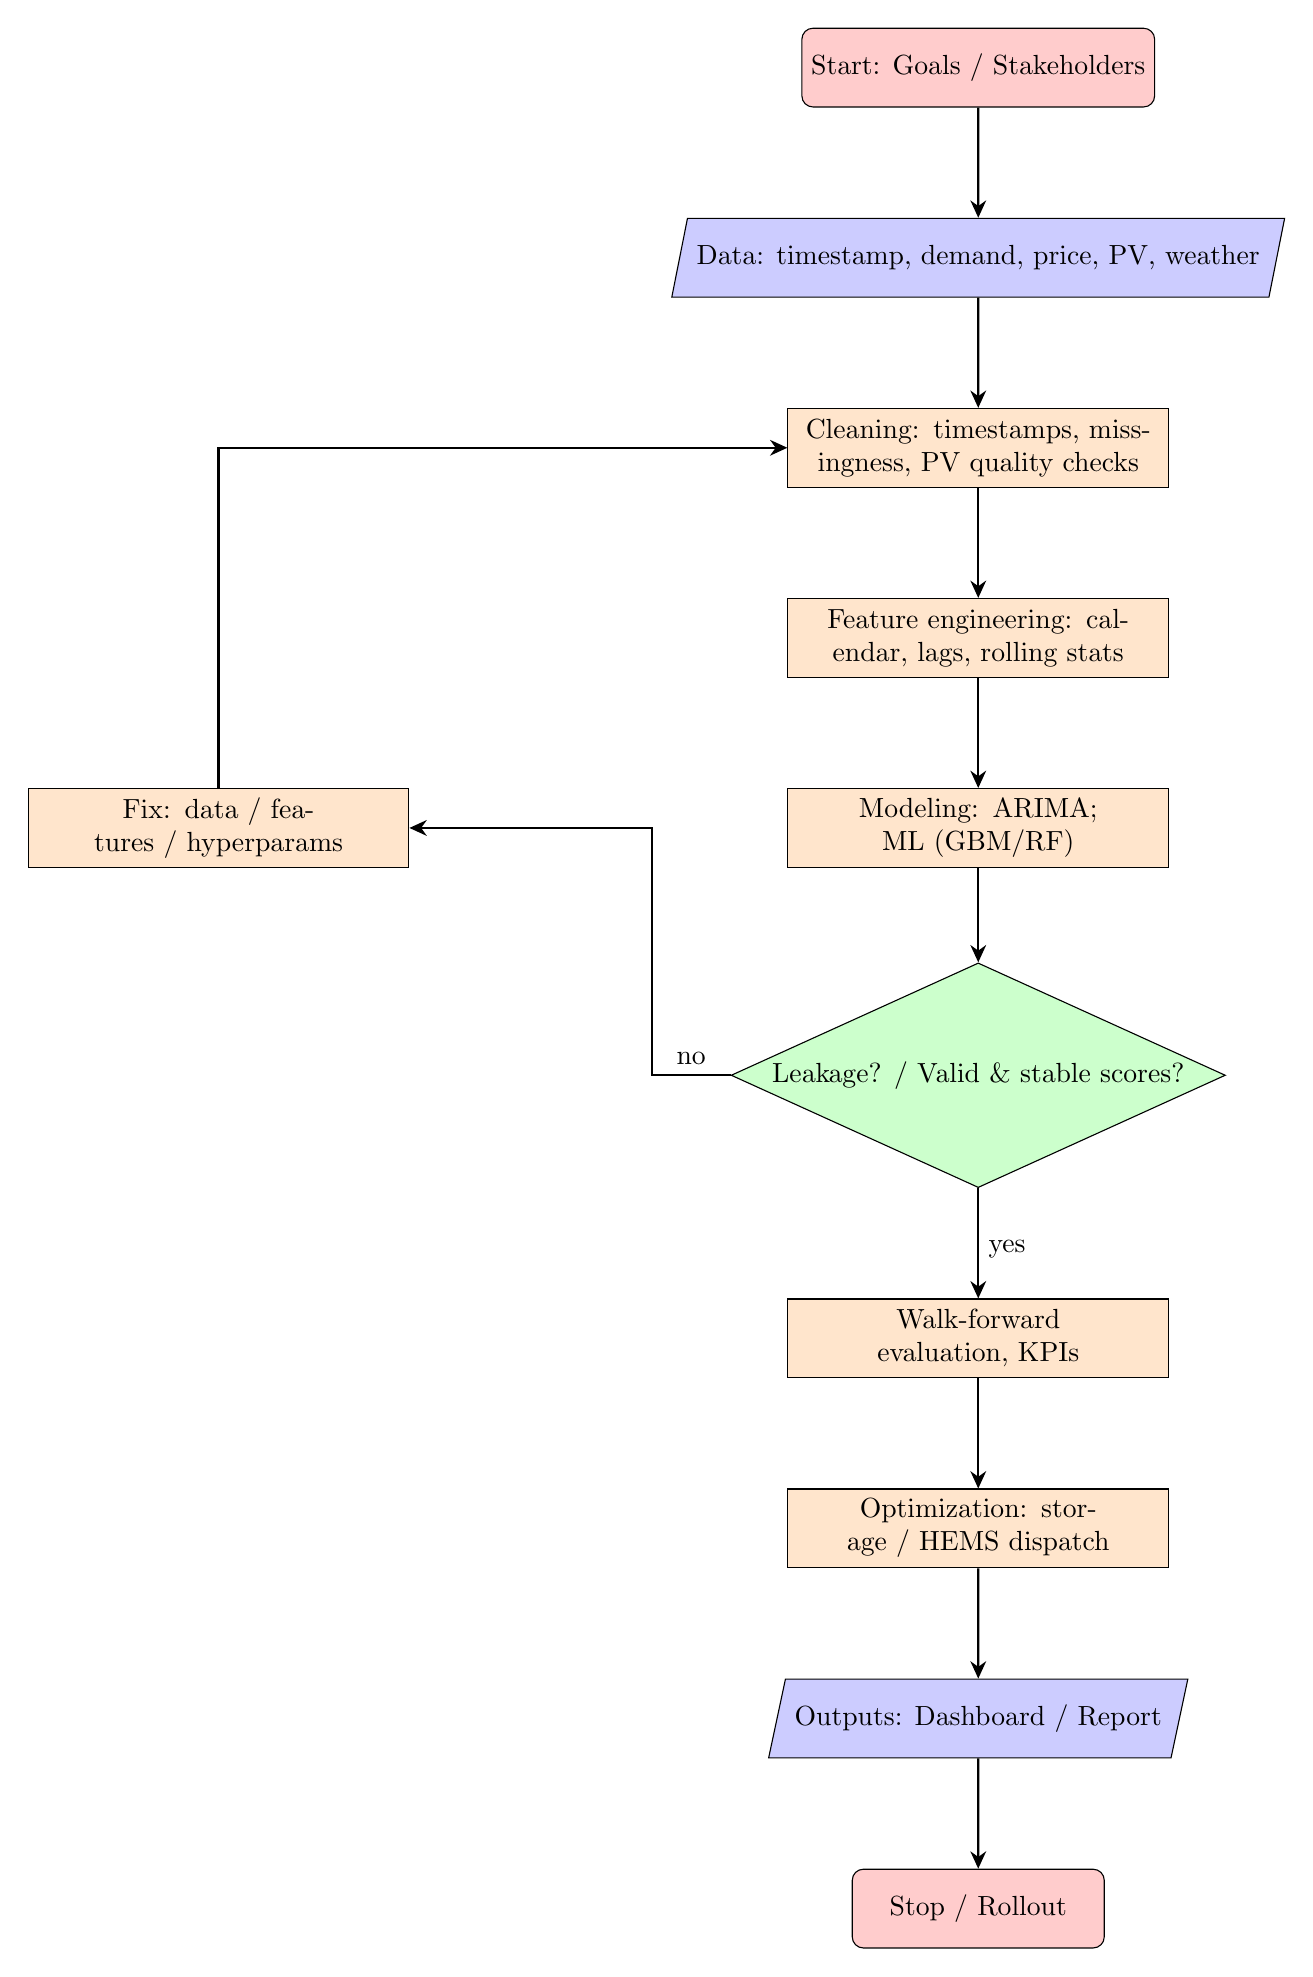
\begin{tikzpicture}[node distance=1.4cm]
    \node (start) [startstop] {Start: Goals / Stakeholders};
    \node (data) [io, below=of start] {Data: timestamp, demand, price, PV, weather};
    \node (prep) [process, below=of data] {Cleaning: timestamps, missingness, PV quality checks};
    \node (feat) [process, below=of prep] {Feature engineering: calendar, lags, rolling stats};
    \node (model) [process, below=of feat] {Modeling: ARIMA; ML (GBM/RF)};
    \node (dec) [decision, below=1.2cm of model] {Leakage? / Valid \& stable scores?};
    \node (eval) [process, below=1.4cm of dec] {Walk-forward evaluation, KPIs};
    \node (opt) [process, below=of eval] {Optimization: storage / HEMS dispatch};
    \node (out) [io, below=of opt] {Outputs: Dashboard / Report};
    \node (stop) [startstop, below=of out] {Stop / Rollout};

    % forward arrows
    \draw[arrow] (start) -- (data);
    \draw[arrow] (data) -- (prep);
    \draw[arrow] (prep) -- (feat);
    \draw[arrow] (feat) -- (model);
    \draw[arrow] (model) -- (dec);
    \draw[arrow] (dec) -- node[right,pos=0.55]{yes} (eval);
    \draw[arrow] (eval) -- (opt);
    \draw[arrow] (opt) -- (out);
    \draw[arrow] (out) -- (stop);

    % feedback branch to avoid overlaps (route to the left)
    \node (fix) [process, left=4.8cm of model] {Fix: data / features / hyperparams};
    \draw[arrow] (dec.west) --++ (-1.0,0) node[above,pos=0.5]{no} |- (fix);
    \draw[arrow] (fix) |- (prep);
  \end{tikzpicture}
  \caption{Project plan (CRISP--DM: Understanding $\to$ Preparation $\to$ Modeling $\to$ Evaluation $\to$ Deployment). Clean layout avoids overlapping connectors.}
  \label{fig:lifecycle}
\end{figure}



\subsection{Expected effort}
We expect the highest effort in \textbf{cleaning and feature engineering} (timestamp/missingness corrections, PV quality checks, robust features), followed by model comparison and walk-forward evaluation. This emphasis aligns with time series practice where preprocessing largely determines forecasting quality \cite{Hyndman2021}.

\subsection{External data sources}
Weather reanalysis (e.g., ERA5) or local observations can improve forecasts; market prices are essential for cost-aware operation. If price and weather are already included in the dataset, additional sources are optional \cite{Hersbach2020}.
%===========================
% 3. Data Exploration
%===========================
\section{Visualisation}

\subsection{Objective and context}
This section visualizes the temporal dynamics and statistical characteristics of the core HEMS variables (demand, PV, price). The objective is to explore the structure, variability, and dependencies of the surface in the diurnal and weekly hours that guide the discovery of features, the detection of anomalies, and the selection of models. Sound visual analysis accelerates the detection of systematic effects (e.g., PV midday peaks, evening demand peaks) and informs preprocessing and modelingchoices \cite{Hyndman2021,Tufte1983}.

\subsection{Statistical overview}
The descriptive statistics for demand, photovoltaic and price are summarized in Table~\ref{tab:task3_stats}. Demand exhibits higher variance during morning and evening peaks, whereas PV shows strong right-skewness due to frequent near-zero night values and intermittent cloud cover. These patterns align with the expected energy profiles of the households and the variability of the sun \cite{Hyndman2021,Antonanzas2016}.

\begin{table}[H]
  \centering
  \caption{Descriptive statistics for Demand, PV, and Price (from \texttt{tables/task3\_summary\_stats.csv}).}
  \label{tab:task3_stats}
  \csvautobooktabular{tables/task3_summary_stats.csv}
\end{table}

\subsection{Visual analysis}
We present complementary visualizations to capture temporal structure, variability, and cross-variable dependence.

\begin{figure}[H]
  \centering
  \includegraphics[width=\linewidth]{figures/task3_fig1_timeseries_overlay.png}
  \caption{Time series overlay (Demand, PV, Price) over a representative week. PV peaks at midday while demand peaks appear in morning/evening; price co-moves with scarcity.}
  \label{fig:task3_ts_overlay}
\end{figure}

\begin{figure}[H]
  \centering
  \includegraphics[width=0.9\linewidth]{figures/task3_fig3_hourly_boxplot.png}
  \caption{Hourly demand boxplots highlighting diurnal variability and evening peaks relevant for storage dispatch.}
  \label{fig:task3_boxplots}
\end{figure}

\begin{figure}[H]
  \centering
  \includegraphics[width=0.95\linewidth]{figures/task3_fig2_distributions.png}
  \caption{Histograms with KDE for Demand and PV showing typical operating ranges and skewness.}
  \label{fig:task3_histograms}
\end{figure}

\begin{figure}[H]
  \centering
  \includegraphics[width=0.8\linewidth]{figures/task3_fig4_correlation_heatmap.png}
  \caption{Correlation heatmap for core variables: positive association between demand and price; midday PV is broadly anti-correlated with net demand.}
  \label{fig:task3_corr}
\end{figure}

\subsection{Interpretation and insights}
The figures reveal strong diurnal and weekday effects (peak demand in morning/evening; PV midday peaks). Correlation patterns motivate feature engineering: calendar variables (hour, weekday), weather covariates (irradiance, temperature), and lagged terms for persistence \cite{Hyndman2021}. Among the plots, the typical hourly structure captured by boxplots and profiles is most informative for downstream HEMS decisions because it concisely indicates when PV–demand mismatches are systematic and sizable, guiding storage control; these visuals adhere to ethical design (clear labels, units, non-deceptive axes) and maximize readability and completeness \cite{Antonanzas2016}.
%===========================
% 4. Data Cleaning
%===========================
\section*{4. Data cleaning}

\subsection*{4.1 Missingness profiling}
We begin with a systematic audit of missingness across the time series. Figure~\ref{fig:task4_missing_heatmap} visualises missing data over time and variables, while Table~\ref{tab:task4_missing_summary} summarises counts and rates. Patterns concentrated at specific periods (e.g., sensor outages) suggest Missing At Random (MAR), while isolated holes may be plausibly Missing Completely At Random (MCAR). When missingness depends on unobserved values (MNAR), simple imputations risk bias \cite{Little2002}.

\begin{figure}[H]
  \centering
  \includegraphics[width=0.95\linewidth]{figures/task4_fig_missing_heatmap.png}
  \caption{Missingness heatmap across variables and time. Clusters indicate outages; isolated gaps may be random losses.}
  \label{fig:task4_missing_heatmap}
\end{figure}

\begin{table}[H]
  \centering
  \caption{Summary of missing values by variable and overall rate.}
  \label{tab:task4_missing_summary}
  \csvautobooktabular{tables/task4_missing_summary.csv}
\end{table}

\subsection*{4.2 Time-of-day and run-length diagnostics}
To detect structural gaps (e.g., firmware resets at fixed hours), we examine missingness by hour-of-day and contiguous run lengths. Figure~\ref{fig:task4_missing_tod} shows missing rate by hour; Table~\ref{tab:task4_missing_tod_tbl} lists per-hour rates. A timeline view (Figure~\ref{fig:task4_missing_timeline}) highlights multi-hour runs that merit careful treatment (e.g., forward-fill caps) rather than naive interpolation.

\begin{figure}[H]
  \centering
  \includegraphics[width=0.8\linewidth]{figures/task4_fig_missing_tod.png}
  \caption{Missingness by hour-of-day (share of samples missing).}
  \label{fig:task4_missing_tod}
\end{figure}

\begin{table}[H]
  \centering
  \caption{Hourly missingness rates.}
  \label{tab:task4_missing_tod_tbl}
  \csvautobooktabular{tables/task4_missing_tod.csv}
\end{table}

\begin{figure}[H]
  \centering
  \includegraphics[width=0.95\linewidth]{figures/task4_fig_missing_timeline.png}
  \caption{Timeline view of missingness runs, revealing outage episodes.}
  \label{fig:task4_missing_timeline}
\end{figure}

\subsection{Imputation strategy and validation}
Given the strong daily structure, we combine conservative forward/backward fills for short gaps with calendar-aware interpolation and, where suitable, model-based imputation using seasonally adjusted series. Figure~\ref{fig:task4_imputation_overlay} overlays raw and imputed series for a representative window; Table~\ref{tab:task4_imputation_summary} reports diagnostic metrics (e.g., gap length distribution, post-imputation variance preservation). We avoid imputing PV at night (kept at zero) and cap fills over long runs to prevent artificial smoothing \cite{Hyndman2021,Little2002}.

\begin{figure}[H]
  \centering
  \includegraphics[width=0.95\linewidth]{figures/task4_fig_imputation_overlay.png}
  \caption{Imputation overlay: raw versus imputations across typical gaps. Strategy preserves diurnal shape while preventing drift.}
  \label{fig:task4_imputation_overlay}
\end{figure}

\begin{table}[H]
  \centering
  \caption{Imputation diagnostics summary.}
  \label{tab:task4_imputation_summary}
  \csvautobooktabular{tables/task4_imputation_summary.csv}
\end{table}

\subsection{Seasonal decomposition as a diagnostic}
Seasonal-Trend decomposition (STL) helps verify that cleaning preserves essential structure. Figure~\ref{fig:task4_stl} shows clean series decomposed into trend, seasonal, and remainder. Seasonal amplitude and stable remainder suggest that imputations did not introduce artifacts and that later ARIMA/ML models can exploit clear seasonality \cite{Hyndman2021}.

\begin{figure}[H]
  \centering
  \includegraphics[width=0.95\linewidth]{figures/task4_fig_stl_components.png}
  \caption{STL components after cleaning: strong diurnal seasonality with reasonable remainder variance.}
  \label{fig:task4_stl}
\end{figure}

\subsection{Daily profiles before and after cleaning}
To verify that imputations did not distort operational patterns, we compare typical daily profiles. Figure~\ref{fig:task4_daily_profiles} indicates that peak timings and amplitudes remain consistent, while extreme outliers are mitigated—desirable for forecasting stability and optimisation downstream.

\begin{figure}[H]
  \centering
  \includegraphics[width=0.9\linewidth]{figures/task4_fig_daily_profiles.png}
  \caption{Typical daily profiles before/after cleaning for demand and PV (median and IQR).}
  \label{fig:task4_daily_profiles}
\end{figure}

\subsection{Limitations and ethical considerations}
While the adopted imputation strategy is conservative, any gap-filling may obscure rare but important behaviours (e.g., extreme peaks). We therefore retain an audit trail of imputed indices and exclude heavily imputed windows from model validation to prevent optimistic bias. From an ethics perspective, cleaning steps avoid fabricating PV at night and preserve physical plausibility. Decisions are documented for reproducibility and to facilitate stakeholder scrutiny \cite{Little2002,Hyndman2021}.



\section{Feature engineering}

\subsection{Objective and overview}
Feature engineering is central to improving predictive performance in short-term demand forecasting. By representing domain structure explicitly---diurnal and weekly cycles, weather sensitivity, persistence---we increase the signal-to-noise ratio that models can exploit \cite{Zheng2020,Hyndman2021}. We leverage three information streams: (i) the demand series (autoregressive lags and rolling summaries), (ii) weather covariates (temperature, solar radiation as proxy for PV), and (iii) calendar variables (hour-of-day, weekday/weekend, month, holidays).

\subsection{Exploratory statistics}
We examine marginal distributions and bivariate relationships to motivate transformations and interactions.

\begin{figure}[H]
  \centering
  \includegraphics[width=0.95\linewidth]{figures/task3_fig2_distributions.png}
  \caption{Histograms with KDE for demand and temperature. Demand shows right-skew due to evening peaks; temperature is often closer to unimodal but may be seasonally shifted.}
  \label{fig:fe_hist_kde}
\end{figure}

\begin{figure}[H]
  \centering
  \includegraphics[width=0.9\linewidth]{figures/03_correlation_heatmap.png}
  \caption{Correlation snapshot among demand, temperature, PV/solar proxies, and price. Temperature typically correlates with demand (heating/cooling), while PV is anti-correlated with net demand at midday.}
  \label{fig:fe_corr}
\end{figure}

\begin{figure}[H]
  \centering
  \includegraphics[width=0.9\linewidth]{figures/03_overlay_demand_pv_price.png}
  \caption{Overlay of demand, PV and price illustrating alignment of peaks and troughs across drivers.}
  \label{fig:fe_overlay}
\end{figure}

Normalit{"a}t: Shapiro--Wilk-Tests auf stichprobenweise Fenster deuten bei Demand h{"a}ufig auf Nicht-Normalit{"a}t (p\,<\,0.05). Zur Stabilisierung der Varianz sind logarithmische oder Box--Cox-Transformationen geeignet, wobei f{"u}r Demand eine shift-Log (nur f{"u}r strikt positive Werte) oder Yeo--Johnson in Betracht kommt; f{"u}r Temperatur ist i. d. R. keine Transformation erforderlich \cite{Hyndman2021}. Transformationen werden nur angewandt, wenn sie die Kalibrierung verbessern und das Interpretationsziel nicht beeintr{"a}chtigen.

\subsection{Feature creation}
Wir erzeugen dom{"a}nenspezifische Zeit- und Wettermerkmale:
\begin{itemize}[leftmargin=1.2em]
  \item \textbf{Kalender:} Stunde (0--23), Wochentag (0--6), Monat (1--12), Wochenende/Feiertag-Indikator. Rationale: f{"a}ngt diurnale und w{"o}chentliche Routinen ein.
  \item \textbf{Autoregressive Lags:} Demand-Lags (1, 2, 24, 48) zur Erfassung von Persistenz und Tagesperiodik.
  \item \textbf{Rollende Statistiken:} Gleitende Mittel/Median (3, 6, 24h) und gleitende Std.-Abweichungen zur Kurzzeitgl{"a}ttung und Volatilit{"a}tssch{"a}tzung.
  \item \textbf{Wetterfeatures:} Temperatur, gef{"u}hlte Temperatur, solare Einstrahlung oder PV als Proxy f{"u}r Helligkeit/Bew{"o}lkung; ggf. Nichtlinearit{"a}ten mittels Bins/Splines.
  \item \textbf{Interaktionen:} PV $\times$ Stunde (Wirksamkeit bei Tag), Temperatur $\times$ Stunde (tageszeitliche Heiz/K{"u}hl-Last), PV $\times$ Temperatur (Bew{"o}lkung und W{"a}rme korreliert).
\end{itemize}
Rationale: Diese Merkmale codieren bekannte physikalische und verhaltensbezogene Mechanismen (Tageslicht, Komfort, Routine) und verbessern die Erkl{"a}rbarkeit.

\subsection{Feature ranking}
Zur Priorisierung nutzen wir korrelationsbasierte Scores und modellbasierte Wichtigkeiten (z.\,B. Random-Forest, Mutual Information). Abbildung~\ref{fig:fe_importance} zeigt die modellbasierte Rangfolge; typischerweise sind Stunde-des-Tages, Temperatur und Vortags-Lags (t-24) am wichtigsten, was die Diurnalit{"a}t und Wetterabh{"a}ngigkeit reflektiert. Falls einige konstruierte Features schwach abschneiden, k{"o}nnen Ursachen Multikollinearit{"a}t (stark korrelierte Lags), {\"U}ber-Engineering (redundante Transformationen) oder zu kurze Historien f{"u}r stabile Sch{"a}tzungen sein \cite{Zheng2020}.

\begin{figure}[H]
  \centering
  \includegraphics[width=0.95\linewidth]{figures/ml_feat_importance.png}
  \caption{Feature-Importance (modellbasiert, z.\,B. Random Forest). Zeitliche Marker (Hour, Day) und Wetter (Temperature/PV) dominieren, Lags tragen Persistenzinformation.}
  \label{fig:fe_importance}
\end{figure}

\subsection{Summary}
Feature Engineering hat den Datensatz f{"u}r statistische Modelle (ARIMA, STL-basiert) und ML-Modelle (GBM, RF) aufbereitet: Diurnalit{"a}t und Wocheneffekte sind explizit, Persistenz wird durch Lags/Rolling-Stats abgebildet, Wetter- und Interaktionsmerkmale erfassen nichtlineare Treiber. Reproduzierbarkeit wird durch skriptbasierte Generierung (Notebook/`src/features.py`) und Versionierung der Feature-Schemata sichergestellt. Validierung erfolgt {\"u}ber Cross-Validation/WFA sowie Drift-Monitoring der Merkmalverteilungen. Gute Praktiken folgen \cite{Zheng2020,Hyndman2021}.

\printbibliography

\end{document}


